\chapterimage{./Pictures/cover-abstract}
\chapter{TP4 : Classes abstraites}
\textit{L'objectif de ce TP numéro 4 est de définir et de manipuler une classe abstraite. Une telle classe ne permet pas d'instancier des objets. Elle sert de classe de base pour un héritage. Les méthodes abstraites sont juste déclarées (les signatures des dites méthodes sont fournies) dans les classes abstraites. Leur définition est donnée dans les classes filles.}

\section{Exercice 1 : Cercle et rectangle}
\textit{L'objectif de cet exercice est de créer deux classes Cercle et Rectangle, ces deux classes ayant de nombreux points communs, il est préférable de créer une classe FormeGeometrique dite "abstraite" donc les deux classes hériteraient.}
\\\\
Je crée dans un premier temps la classe abstraite FormeGeometrique, voici son code :
\inputminted[linenos,firstline=3,lastline=23]{java}{../sources/src/tp4/FormeGeometrique.java}
Cette classe est une classe abstraite nous ne pouvons pas l'instancier comme nous instancierons une classe normal :
\begin{minted}{java}
FormeGeometrique forme = new FormeGeometrique(1.0);
\end{minted}
Cependant nous pouvons instancier une classe anonyme de cette facon :
\begin{minted}{java}
FormeGeometrique forme = new FormeGeometrique(1.0) {
            @Override
            public double calculPerimetre() {
                return 0;
            }

            @Override
            public double calculSuperficie() {
                return 0;
            }

            @Override
            public String toString() {
                return "$classAnonymous{" +
                        "epaisseur=" + epaisseur +
                        '}';
            }
        };
\end{minted}

Je crée ensuite les classes Cercle et Rectangle de cette manière :
\inputminted[linenos,firstline=3,lastline=33]{java}{../sources/src/tp4/Cercle.java}

\inputminted[linenos,firstline=3,lastline=38]{java}{../sources/src/tp4/Rectangle.java}

Ces deux classes ne sont pas abraites et les méthodes sont bien redéfinies, il est donc possible de les instancier.

\section{Exercice 2 : Tableau de formes géométriques}
\textit{L'objectif de cet exercice est de créer un tableau de formes géométriques, on pourra ainsi voir l'intérêts supplémentaires de l'héritage et des classes abstraites.}
\\\\
Je crée donc une classe TableauFormeGeometrique, avec comme attribut un nombre de forme ainsi qu'une liste contenant des formes géométriques.
Voici le code de la classe TableauFormeGeometrique :
\inputminted[linenos,firstline=6,lastline=36]{java}{../sources/src/tp4/TableauFormeGeometrique.java}

Voici le code de la classe Main :
\inputminted[linenos,firstline=3,lastline=38]{java}{../sources/src/tp4/Main.java}

Le fait d’avoir créé une classe abstraite FormeGeometrique nous permet de stocker dans ce notre tableau des cercles et des rectangles puisque les deux héritent de FormeGéométrique, c’est l’un des intérêts des classes abstraites.

À l'éxecution On obtient l’affichage final suivant :
\begin{figure}[H]
  \centering
  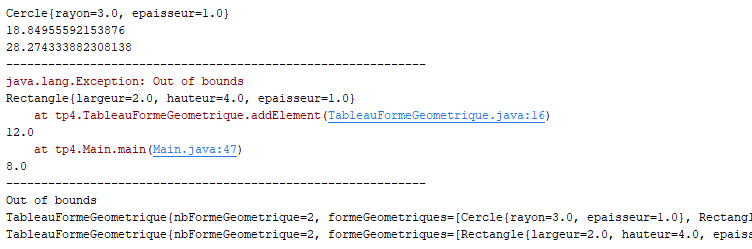
\includegraphics[width=500pt]{./tp/Pictures/tp4-execute}
  \caption{Exécution TP4}
  \label{Exécution TP4}
\end{figure}
